\documentclass{article}

\begin{document}

\usepackage{titlesec}
\usepackage{graphicx}


\title{Apo-Rodagon-N}
\section{Manufacturer}
Rodenstock
\section{Focal Lengths}
50mm, 80mm, 105mm   
\section{Information}

For the use of these lenses as taking lenses for close up and macro photography with 35 mm SLR cameras as well as for use as high resolution taking lenses with CCD still and video cameras, the same applies as to the use of the Rodagon; how-ever, the definition and the brilliance is still a little bit better.

\section{Recommended Magnification}
2x-15x
\section{Price}

ebay: 300-600€

\begin{figure}
\centering
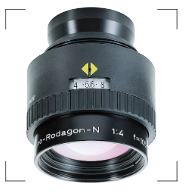
\includegraphics[width=\textwidth]{apo-rodagon-n-1.png}
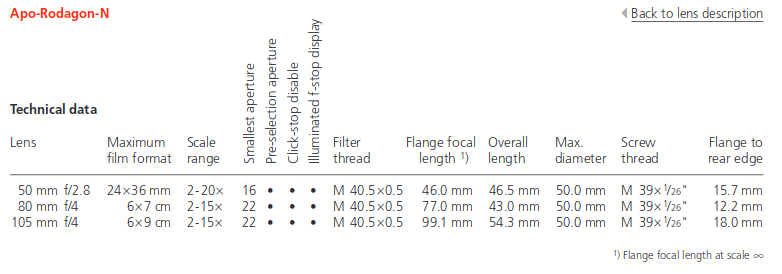
\includegraphics[width=\textwidth]{apo-rodagon-n-2.png}
\end{figure}


\end{document}
